\documentclass[tikz,border=6pt]{standalone}
% Shared look for the Details diagrams: the site's cave palette on a
% transparent ground, so the SVG sits on the dark page with no box around it.
\usepackage[T1]{fontenc}
\usepackage{helvet}
\usepackage{amsmath,amssymb}
\renewcommand{\familydefault}{\sfdefault}
\usetikzlibrary{arrows.meta,positioning,calc,backgrounds,fit}
\definecolor{ink}{HTML}{D7DBE0}
\definecolor{dim}{HTML}{99A1AD}
\definecolor{faint}{HTML}{6D7682}
\definecolor{rock}{HTML}{21262E}
\definecolor{edge}{HTML}{4A525E}
\definecolor{lamp}{HTML}{7AA2F7}
\definecolor{gold}{HTML}{F5B301}
\definecolor{moss}{HTML}{4AA06A}
\definecolor{ember}{HTML}{E05A4D}
\tikzset{
  every node/.style={text=ink},
  flow/.style={-{Stealth[length=2.4mm]}, line width=0.8pt, draw=dim},
  call/.style={-{Stealth[length=2mm]}, line width=0.7pt, draw=gold, dashed},
  lab/.style={font=\scriptsize, text=dim, align=center, inner sep=1.5pt},
}

\begin{document}
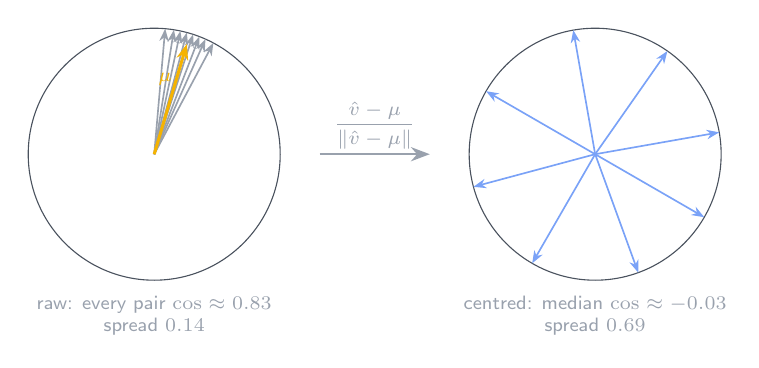
\begin{tikzpicture}
% left: raw vectors in a narrow cone
\begin{scope}
  \draw[edge] (0,0) circle (1.6);
  \foreach \a in {62,66,69,72,75,78,81,85} \draw[dim, line width=0.6pt, -{Stealth[length=1.6mm]}] (0,0) -- (\a:1.6);
  \draw[gold, line width=1.1pt, -{Stealth[length=2mm]}] (0,0) -- (73.5:1.46);
  \node[lab, text=gold, anchor=east] at (73.5:1.0) {$\mu$};
  \node[lab, align=center] at (0,-2.05) {raw: every pair $\cos\approx0.83$\\spread $0.14$};
\end{scope}
\draw[flow] (2.1,0) -- node[lab, above] {$\dfrac{\hat v-\mu}{\lVert\hat v-\mu\rVert}$} (3.5,0);
% right: centred vectors spread round the circle
\begin{scope}[xshift=5.6cm]
  \draw[edge] (0,0) circle (1.6);
  \foreach \a in {10,55,100,150,195,240,290,330} \draw[lamp, line width=0.6pt, -{Stealth[length=1.6mm]}] (0,0) -- (\a:1.6);
  \node[lab, align=center] at (0,-2.05) {centred: median $\cos\approx-0.03$\\spread $0.69$};
\end{scope}
\end{tikzpicture}
\end{document}
